\section{Recursive structure}\label{sec:recursion}

A successful natural language inference system must reason 
about relations not just over familiar
atomic symbols, but also over novel structures built up 
recursively from these symbols. 
This section shows that our models can learn a 
compositional semantics over such structures.
In our evaluations, we exploit the fact that our logical language
is infinite by testing on strings that are longer and more complex
than any seen in training.

% Consider, for example, \ii{Alice said hello}, \ii{Bob said that Alice
%   said hello}, and \ii{Carl thinks that Bob said that Alice said
%   hello}. Overt recursion of this kind is easy to find, and
% theoretical accounts of natural language syntax and semantics rely
% heavily on recursive structures. In order for a model to be able to
% accurately learn natural language meanings, then, we expect that it
% would need to be able to learn to represent the meanings of function
% words in a such a way that they are able to behave correctly when
% taking their own outputs as input. In evaluating the model, we take
% advantage of the fact that recursive structures of this kind define
% potentially infinite languages by testing the model on strings that
% are longer and more complex than any seen in testing.

\paragraph{Experiments}
As in \S\ref{sec:join}, we generate artificial data from a formal system,
 but we now replace the unanalyzed symbols
from that experiment with complex formulae. These formulae
represent a complete classical propositional logic:
each atomic symbol is a variable over the domain \{$\True$, $\False$\}, and the only
operators are truth-functional ones.  Table~\ref{tab:pl} defines this
logic, and Table~\ref{tab:plexs} gives some short examples of relational statements from our data.
 To compute these relations
between statements, we exhaustively enumerate the sets of assignments
of truth values to propositional variables that would satisfy each of
the statements, and then we convert the set-theoretic relation between
those assignments into one of the seven relations in
Table~\ref{b-table}. As a result, each relational statement represents
a valid theorem of the propositional logic, and to succeed, the models 
must learn to reproduce the behavior of a theorem prover.\footnote{
Socher et al.~\shortcite{socher2012semantic} show that a matrix-vector TreeRNN
model somewhat similar to our TreeRNTN can learn boolean logic, 
a logic where the atomic symbols are simply the
values $\True$ and $\False$. While learning the operators of that logic is not trivial, the outputs of
each operator can be represented accurately by a single bit.
In the much more demanding task presented here, the atomic symbols are variables over these values, and the sentence vectors must thus be able to distinguish up to $2^{64}$ distinct conditions on valuations.}

\begin{table}[tp]
  \centering\small
  \begin{subtable}[t]{0.45\textwidth}
    \centering
    \begin{tabular}[t]{l l}
      \toprule
      Formula     & Interpretation \\
      \midrule
      $p_1$, $p_2$, $p_3$, $p_4$, $p_5$, $p_6$ & $\sem{x} \in \{\True, \False\}$ \\
      $\plneg \varphi$ & $\True$ iff $\sem{\varphi} = \False$ \\
      $(\varphi \pland \psi)$ & $\True$ iff $\False \notin \{\sem{\varphi}, \sem{\psi}\}$ \\
      $(\varphi \plor \psi)$  & $\True$ iff $\True \in \{\sem{\varphi}, \sem{\psi}\}$ \\
      \bottomrule
    \end{tabular}    
    \caption{Well-formed formulae. $\varphi$ and $\psi$
      range over all well-formed formulae, and $\sem{\cdot}$ is
      the interpretation function mapping formulae into $\{\True,
      \False\}$.}\label{tab:pl}
  \end{subtable}
  \begin{subtable}[t]{0.45\textwidth}
    \centering\vspace{4mm}
    \begin{tabular}[t]{r c l}
      \toprule
      $\plneg p_3$        & $\natneg$ & $p_3$ \\
      $\plneg \plneg p_6$ & $\nateq$  & $p_6$ \\
      $p_3$               & $\natfor$ & $(p_3 \plor p_2)$ \\
      $(p_1 \plor (p_2 \plor p_4))$               & $\natrev$ & $(p_2 \pland  \plneg p_4)$ \\
      %$(a \natfor b)$   & $\nateq$  & $(b \natrev a)$ \\	
      $\plneg\, (\plneg p_1 \pland \plneg p_2)$ & $\nateq$ & $(p_1 \plor p_2)$ \\ 
      \bottomrule
    \end{tabular}
    \caption{Examples of the type of statements used for training and testing. These are relations between
      well-formed formulae, computed in terms of sets of satisfying
      interpretation functions $\sem{\cdot}$.}\label{tab:plexs}
  \end{subtable}
  \caption{Natural logic relations over sentences of propositional logic.}  
  \label{prop-figure}
\end{table}

In our experiments, we randomly generate unique pairs 
of formulae containing up to 12 instances of logical operators each and compute the relation that holds for each pair.
We discard pairs in which either statement is either a tautology or a
contradiction, for which the seven relations in
Table~\ref{b-table} are undefined. The resulting set of formula pairs is
then partitioned into 12 bins according the number of operators in
the larger of the two formulae. We then sample 20\% of each
bin for a held-out test set.
If we do not implement any constraint that the two statements being
compared are similar in any way, then the generated data are dominated
by statements in which the two formulae refer to largely separate
subsets of the six variables, which means that the $\natind$ relation
is almost always correct.  In an effort to balance the distribution of
relation labels without departing from the basic task of modeling
propositional logic, we disallow individual pairs of statements from
referring to more than four of the six propositional variables.

In order to test the model's generalization to unseen structures, we discard
training examples with more than 4 logical operators, yielding 60k short training examples,
and 21k test examples across all 12 bins.
In addition to the two tree models, we also train a summing NN baseline
which is largely identical to the TreeRNN, except that instead of using a learned composition function,
it simply sums the term vectors in each expression to compose them before passing them to the comparison layer. Unlike the two tree models, this baseline does not use word order,
and is as such guaranteed to ignore some information that it would need in order to succeed perfectly.

\begin{figure}[t]
  \centering
  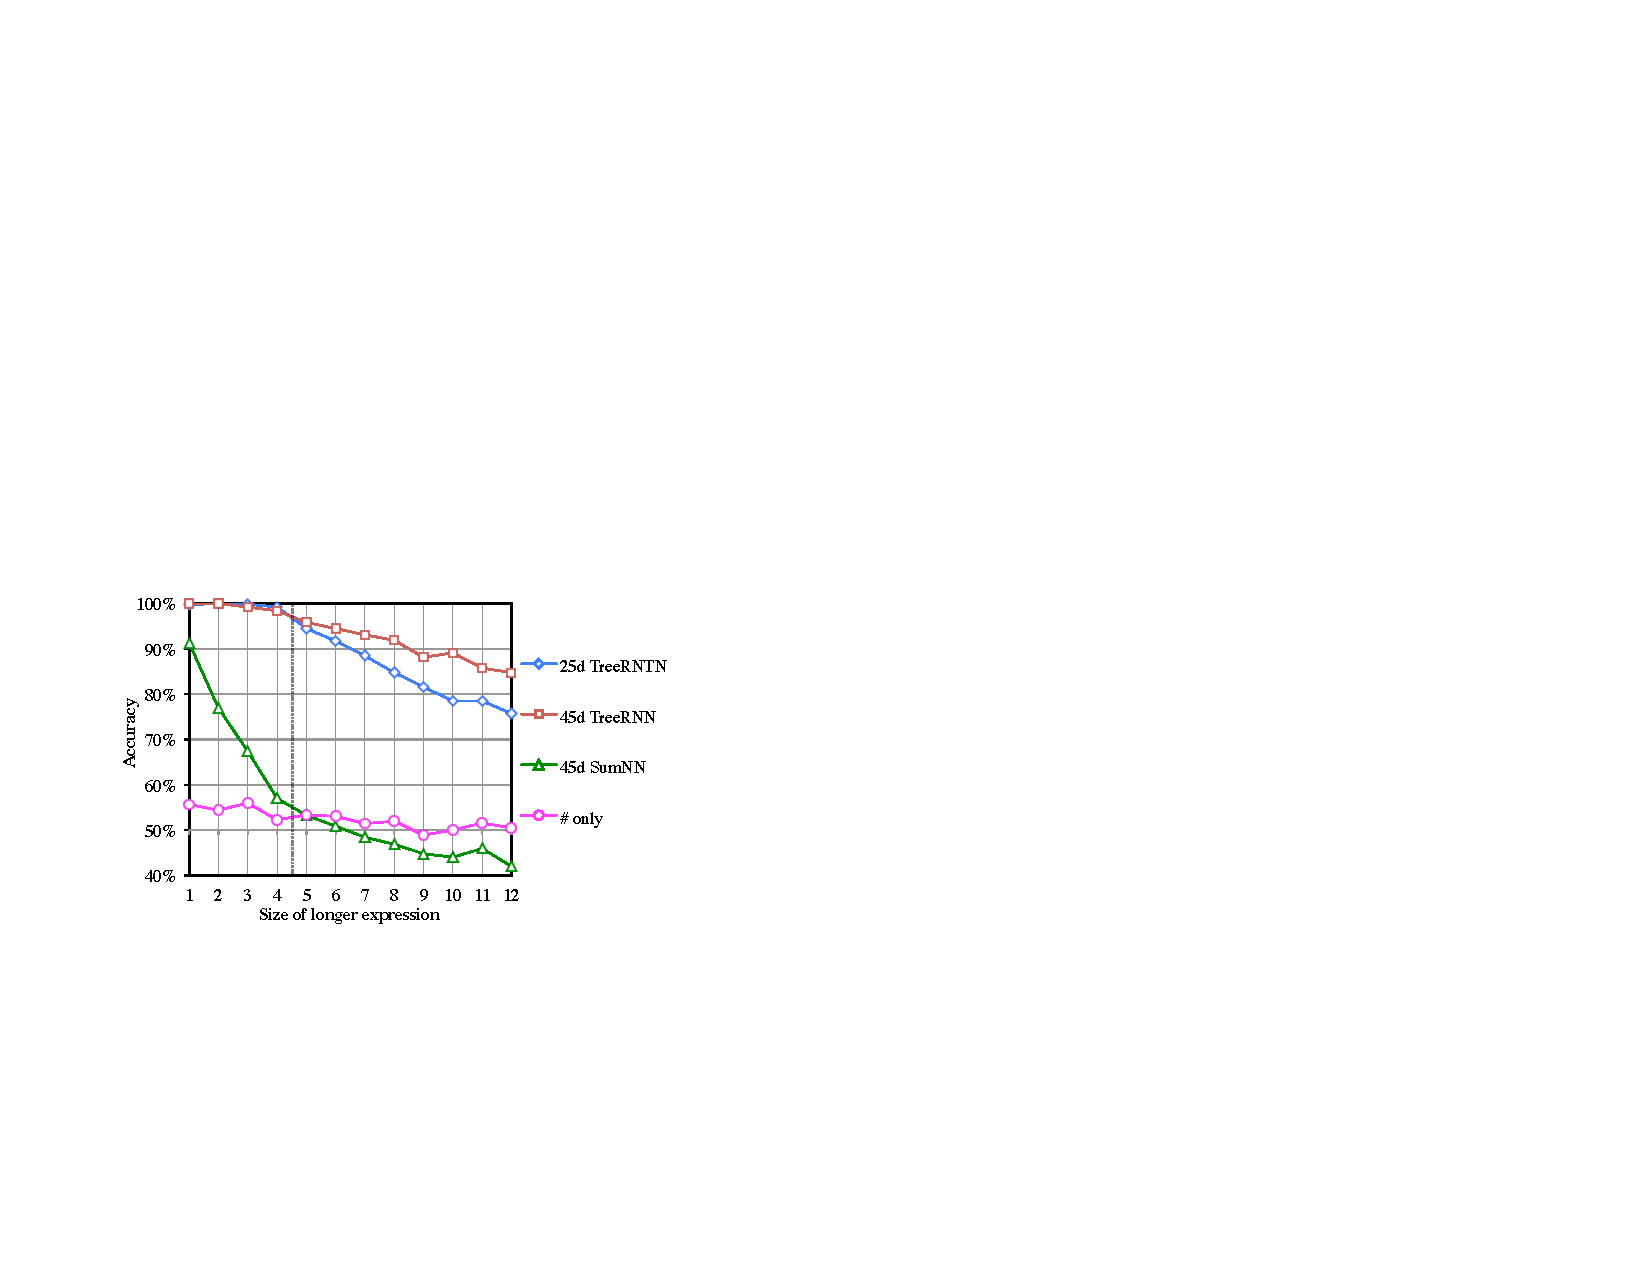
\includegraphics[width=3.05in]{decayfig.pdf}
%  \includegraphics[width=5.3in]{recursion\string_pairwise.eps}
  \caption{Results on recursive structure. The vertical dotted line marks the size of the longest training examples.}
%    The dashed line indicates that only expressions of size four or less appeared in the training data. \textbf{Bottom:} Semantically distinct formulae should have different
%    representations. As measured by Euclidean distance, only the TreeRNTN
%    achieves this for formulae containing more than a small number of
%    connectives (\ii{and} in this example). The TreeRNN quickly collapses the representations,
%    failing to capture the meaning contrasts.
    
  \label{prop-results} 
\end{figure}


\paragraph{Results} Fig.~\ref{prop-results} shows the relationship
between test accuracy and statement size. While the summing baseline model performed poorly across the board, we found that both recursive
models were able to perform well on unseen small test examples, 
with TreeRNN accuracy above
98\% and TreeRNTN accuracy above 99\% on formulae below length five, indicating
that they learned correct approximations of the underlying
logic. Training accuracy was 66.6\% for the SumNN, 99.4\% for the TreeRNN, and 99.8\% for the TreeRNTN.

After the size four training cutoff, performance gradually decays with expression size for both tree models, suggesting that the learned approximations were accurate but lossy.
Despite the TreeRNTN's stronger performance on short sentences, its performance
decayed more quickly than the TreeRNN's. 
This suggests to us that it learned to interpret many specific fixed-size tree structures directly,
allowing it to get away without learning as robust generalizations about how to compose
terms in the general case.
Two factors may have contributed to the learning of these narrower generalizations: 
even with the lower dimension,
the TreeRNTN composition function has about eight times as many parameters as the
TreeRNN, and the TreeRNTN worked best with weaker L2 regularization than the 
TreeRNN ($\lambda = 0.0003$ vs. $0.001$). 
However, even in the most complex set of test examples, the TreeRNTN classifies true examples of every
 class but $\nateq$ (which is rare in long examples, and occurs only once here) correctly 
the majority of the time, and
 the performance of both models on those examples indicates that both have learned
  reasonable approximations of the underlying theorem proving task over recursive structure.

% \mynote{In an effort to better understand why model performance decays, 
%we evaluated both models on pairs of long formulae involving
%binary connectives, to assess how well they distinguish representations for semantically distinct
%formulae. We found that only the TreeRNTN is able to learn
%substantially different representations for pairs of differing formulae like $(a \pland (a \pland a))$
% and $(a \pland (a \pland b))$ when the difference between the two is placed under multiple operators.
%The TreeRNN separates the bare symbols by a euclidean distance of 3.5, but this falls to less than one once the two are placed under three operators, and quickly approaches zero as depth increases.
% The TreeRNTN separates the bare symbols by 2.5, and this falls off much more gradually to 1.3 with twelve operators.}

% we discovered that this model looses information about in longer
% statements in a particularly problematic way. It appears that that
% model is unable to distinguish between two sentences when the only
% difference between those sentences is embedded within a very deep
% structure. We evaluated both models on sentences that differed in only
% one term, but for which that one term was embedded under a large
% number of conjunctions, such as the pair \ii{a (and a)} and \ii{a (and
%   b)}, or the pair \ii{a (and (a (and a)))} and \ii{a (and (a (and
%   b)))}. We then measured the Euclidean distance between the vector
% representations of the two sentences in each pair. Our findings are
% shown in Figure~\ref{prop-falloff}, and show that while the TreeRNTN can
% distinguish the two sentences well at every size that we test, the TreeRNN
% fails after a depth of approximately six.


